\chapter{模拟实验与结果分析}
本章将基于所构建的人工市场系统,对网络暴力机制的行为演化过程与经济后果进行数值模拟与实证分析。为探究网络暴力在社交网络中传播如何影响市场参与者的行为决策及市场宏观特征,实验设计了如下两种主要情景:

\begin{itemize}
  \item \textbf{基础情景(Baseline)}:不引入网络暴力模块,仅保留市场结构与异质投资者行为,用于作为对照参照;
  \item \textbf{网络暴力情景(Cyberbullying)}:启用网络暴力传播模块,在散户之间构建社交网络,模拟言语攻击行为的传导、反馈及行为偏差。
\end{itemize}

两类情景均在相同的市场结构与交易规则下运行,唯一差异为是否启用网络暴力相关模块。每种情景下,仿真时间长度设定为 \( T = 50000 \) 个时间步,并重复运行 \( M = 10 \) 次以确保结果的稳健性。所有模拟采用统一随机种子框架,确保可重复性。

模型的详细参数设定包括市场参数、投资者行为参数、网络结构参数以及传播与反馈机制参数。为节省正文篇幅,完整参数表已整理至附录~\ref{appendix:params},实验中的关键参数设置将在图表说明中简要列出。

接下来将从模型有效性验证、投资者财富影响以及市场效率扰动三个角度依次展开模拟结果的展示与分析。   


\section{模型有效性验证}

在正式分析网络暴力机制影响之前,有必要首先验证所构建的人工市场系统是否能够复现实实市场中常见的统计特征,即"stylized facts"。本节将从价格行为、收益率分布、波动性结构等方面展开验证,重点考察模型在基础情景(Baseline)下的市场统计特性是否合理,以及网络暴力机制引入后市场行为是否发生显著变化。

\subsection{价格走势比较}

图~\ref{fig:price_evolution} 展示了两种情景下模拟市场价格的时间演化路径。可以看到,虽然两者长期走势趋势大致一致,但在 Cyberbullying 情景下,价格路径整体更加震荡,振幅更大,尤其在后期呈现出明显的高频波动,显示出更强的短期不稳定性。与之相比,Baseline 情景下价格曲线更加平滑,波动幅度相对较小。

\begin{figure}[htbp]
    \centering
    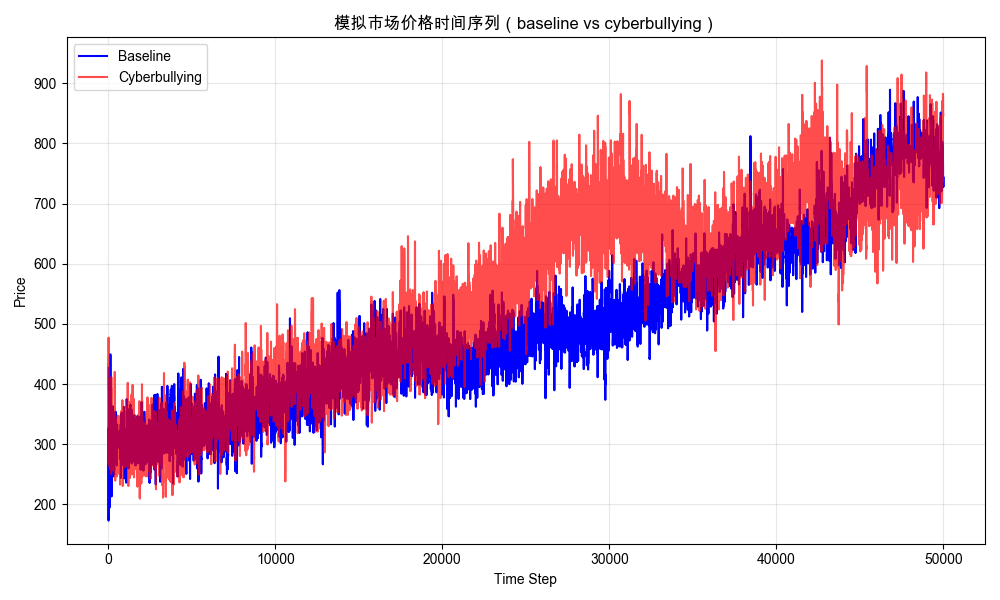
\includegraphics[width=0.95\textwidth]{image/fig4_1_price_evolution.png}
    \caption{模拟市场价格时间序列}
    \label{fig:price_evolution}
\end{figure}

\subsection{收益率分布}

图~\ref{fig:return_hist} 和图~\ref{fig:return_qq} 分别展示了两种情景下的对数收益率分布直方图与 QQ 图。可以观察到,收益率分布在两个情景下均呈现典型的尖峰厚尾特征,显著偏离正态分布。在 Cyberbullying 情景下,收益分布更加扁平、尾部更厚,极端收益事件出现频率更高,反映出更强的风险性。

QQ 图进一步验证了这种非正态性,两个情景下的收益率分位点均呈现出明显的 S 形偏离趋势,尤其 Cyberbullying 更加显著,说明模型生成的市场数据具备现实金融市场的统计特征。

\begin{figure}[htbp]
    \centering
    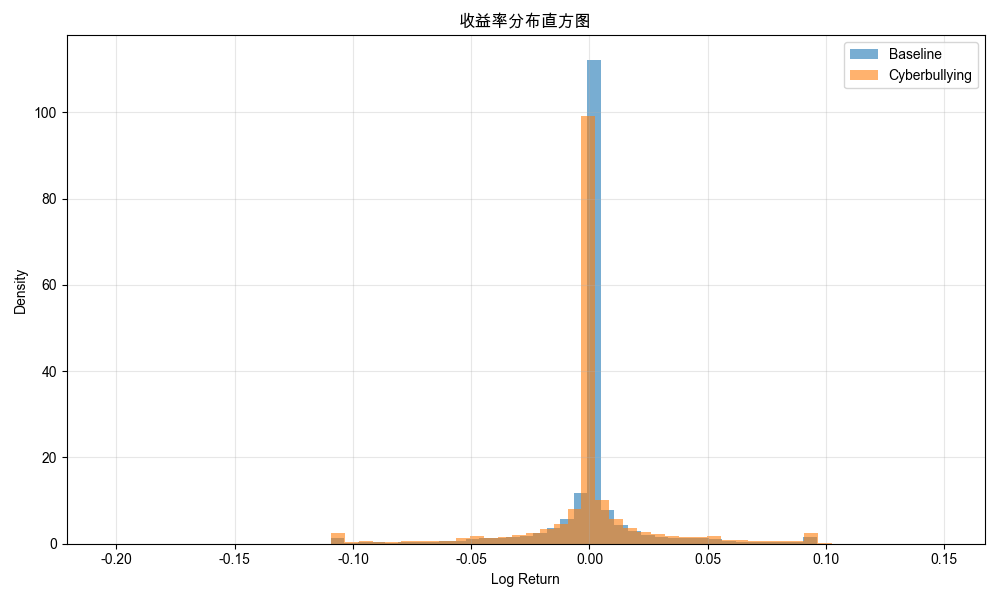
\includegraphics[width=0.85\textwidth]{image/fig4_2_return_hist.png}
    \caption{收益率分布直方图}
    \label{fig:return_hist}
\end{figure}

\begin{figure}[htbp]
    \centering
    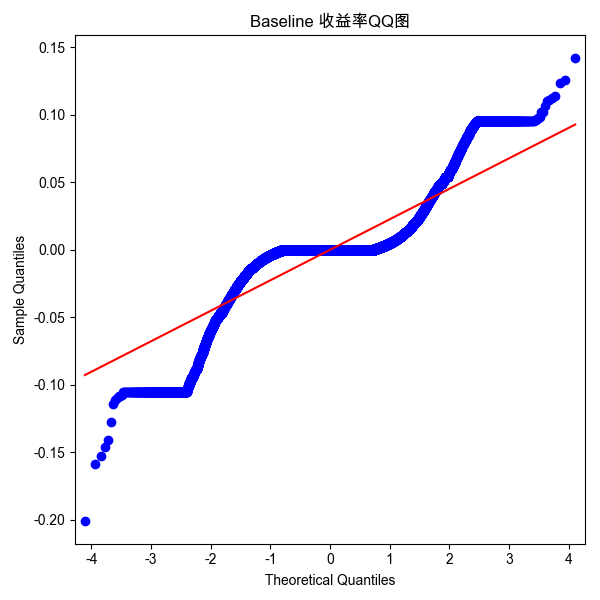
\includegraphics[width=0.48\textwidth]{image/fig4_3_return_qq_baseline.png}
    \hfill
    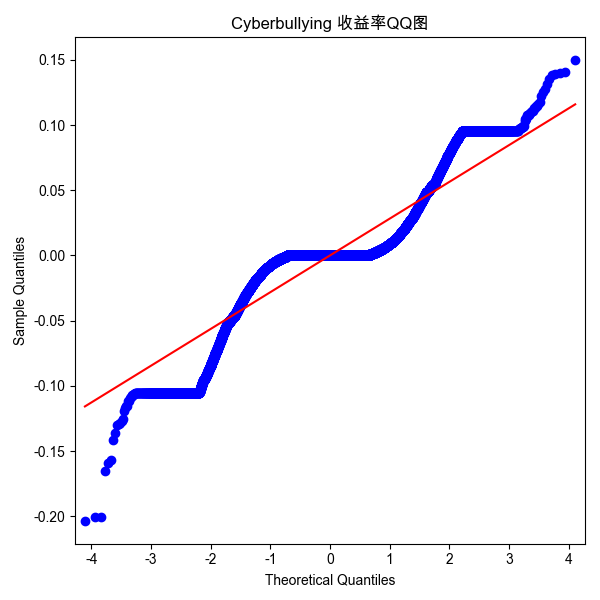
\includegraphics[width=0.48\textwidth]{image/fig4_3_return_qq_cyberbullying.png}
    \caption{收益率 QQ 图(左:Baseline,右:Cyberbullying)}
    \label{fig:return_qq}
\end{figure}

表~\ref{tab:return_stats} 列出了两种情景下对数收益率的统计量。可以看出,在 Cyberbullying 情景中,收益率的标准差和峰度均显著高于 Baseline,进一步说明网络暴力机制的引入使市场的收益波动性增强,厚尾特征加剧。

\begin{table}[htbp]
\renewcommand{\arraystretch}{1.4}
\centering
\large
\begin{threeparttable}
\begin{tabular}{@{} >{\centering\arraybackslash}p{3.5cm}
                >{\centering\arraybackslash}p{2.5cm}
                >{\centering\arraybackslash}p{2.5cm}
                >{\centering\arraybackslash}p{2.5cm}
                >{\centering\arraybackslash}p{3.0cm} @{}}
\toprule\toprule
\textbf{情景} & \textbf{均值} & \textbf{标准差} & \textbf{偏度} & \textbf{峰度} \\
\midrule
Baseline & 0.00006 & 0.0117 & -0.05 & 4.81 \\
Cyberbullying & 0.00004 & 0.0143 & -0.19 & 6.52 \\
\bottomrule\bottomrule
\end{tabular}

\vspace{1em}

\begin{tablenotes}
\item[] 注:各统计量基于对数收益率序列计算,峰度值高于正态分布的 3 表明存在厚尾性;Cyberbullying 情景下标准差与峰度进一步上升,说明市场波动性加剧。
\end{tablenotes}

\caption{收益率统计量比较表}
\label{tab:return_stats}
\end{threeparttable}
\end{table}

\subsection{波动率聚集现象}

图~\ref{fig:return_acf} 给出了 Baseline 情景下对数收益率绝对值的自相关函数(ACF)。结果显示,虽然原始收益率接近白噪声,但其绝对值序列在多个滞后期均存在显著正相关,表明市场波动具有聚集性。随着时间步数延长,这一现象更为清晰,体现出模型在波动结构上的合理性。

\begin{figure}[htbp]
    \centering
    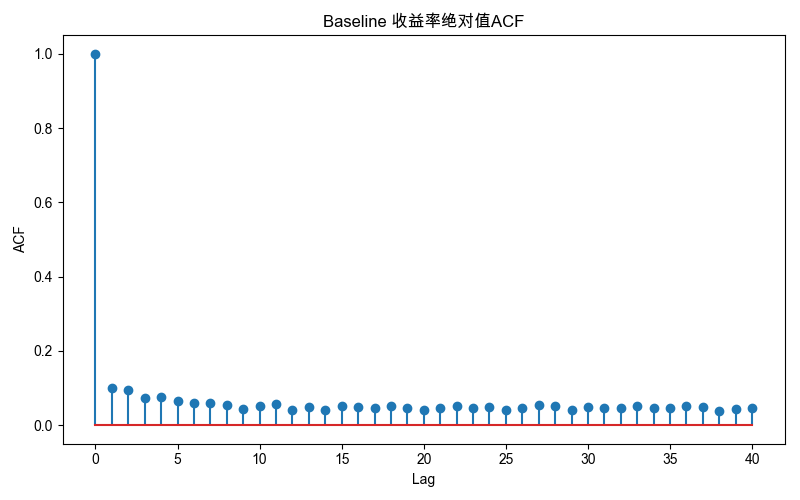
\includegraphics[width=0.7\textwidth]{image/fig4_4_return_acf_baseline.png}
    \caption{Baseline 情景下收益率绝对值的自相关函数(ACF)}
    \label{fig:return_acf}
\end{figure}

综上,仿真结果表明本模型能够在较长时间尺度上稳定复现实实市场中的统计特征,且网络暴力机制的引入在收益率分布、价格波动幅度等维度上对市场稳定性产生显著扰动。这为后续深入分析网络暴力对投资者行为与市场效率的影响奠定了行为基础。






\section{网络暴力对投资者财富的影响}

网络暴力不仅干扰投资者的情绪表达,还会对其交易行为、风险承担能力和市场参与意愿造成深远影响,进而改变其财富演化路径。本节将从投资者身份、攻击状态、不平等性三个方面系统分析网络暴力对个体和群体财富分布所产生的影响,并结合配对 \(t\) 检验检验其统计显著性。

实验采用固定初始种子下对 baseline 与 cyberbullying 两种情景进行一一配对仿真,记录各类投资者在终期的财富水平,并进行组间对比分析。

\subsection{不同类型投资者的财富变化}

图~\ref{fig:final_wealth_boxplot_combined} 展示了机构投资者与散户在 baseline 与 cyberbullying 情景下的终期财富分布对比。
机构投资者的中位数虽在 cyberbullying 情景下略有下降,但分布结构基本一致,标准差无明显变化,配对 \(t\) 检验亦不显著(\(p = 0.69\))。这说明机构作为低情绪敏感群体,对网络暴力机制具备较强的免疫力。
相比之下,散户投资者的中位财富在引入网络暴力机制后显著下降,整体分布左移且收缩明显,表现出普遍性损失。该结果表明网络暴力抑制了部分散户的正常交易行为,使其在长期中积累财富的能力受到削弱。




\begin{figure}[htbp]
    \centering
    \begin{subfigure}[t]{0.48\textwidth}
        \centering
        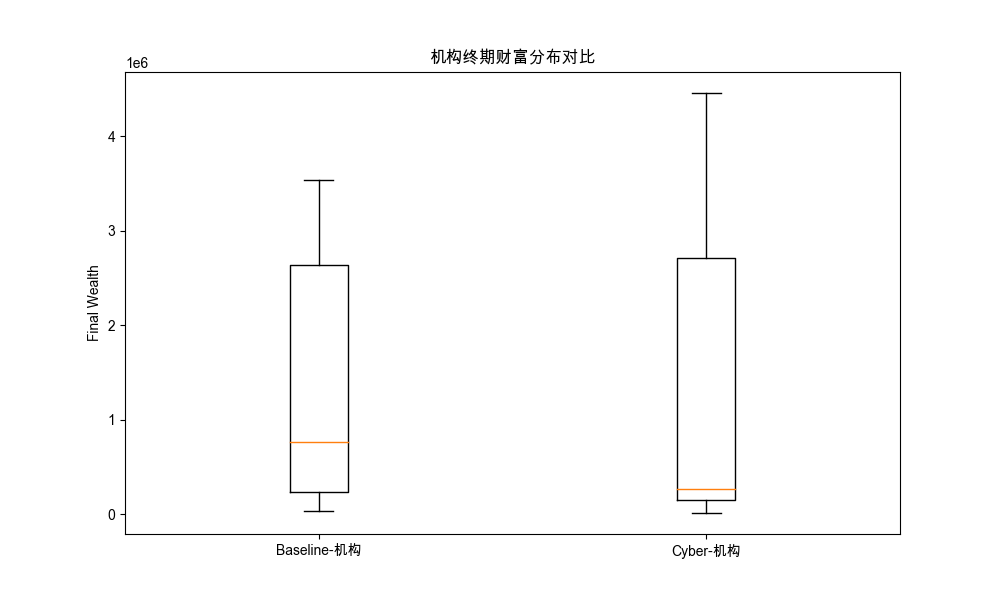
\includegraphics[width=\textwidth]{image/fig4_5_final_wealth_boxplot_institutional.png}
        \caption{机构投资者终期财富分布}
        \label{fig:final_wealth_boxplot_institutional}
    \end{subfigure}
    \hfill
    \begin{subfigure}[t]{0.48\textwidth}
        \centering
        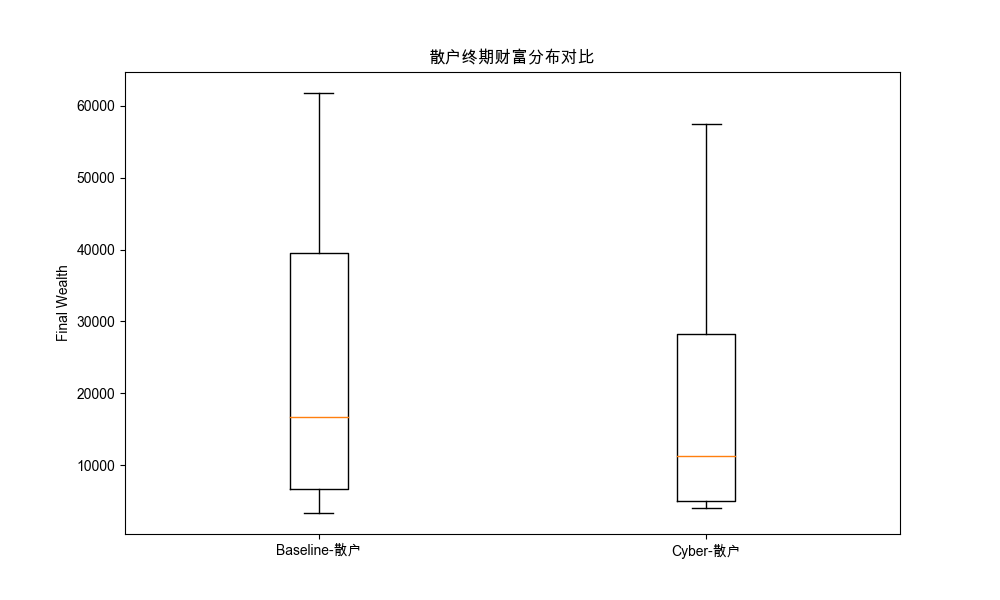
\includegraphics[width=\textwidth]{image/fig4_5_final_wealth_boxplot_retail.png}
        \caption{散户投资者终期财富分布}
        \label{fig:final_wealth_boxplot_retail}
    \end{subfigure}
    \caption{不同类型投资者终期财富分布对比(Baseline vs Cyberbullying)}
    \label{fig:final_wealth_boxplot_combined}
\end{figure}


\subsection{攻击状态分组分析}

为了进一步理解网络暴力的作用路径,本节将散户群体按是否在 cyberbullying 情景中遭受攻击划分为"被攻击者"与"未被攻击者",并将其与 baseline 下的散户财富分布进行对比。

图~\ref{fig:attacked_vs_not_boxplot} 显示,被攻击者的终期财富大幅下降,分布收缩至低水平区域,部分个体几乎损失全部资产,显示情绪压制已显著削弱其市场存续能力。而未被攻击的散户不仅财富中位数高于 baseline,且分布更广,可能从波动性增加中获利。

该现象反映了网络暴力机制的"选择性效应":在相同市场机制下,部分投资者由于受到攻击而情绪压制、退出交易;而另一些未受攻击者则在风险加剧环境下更积极参与,从而获取额外收益。

\begin{figure}[htbp]
    \centering
    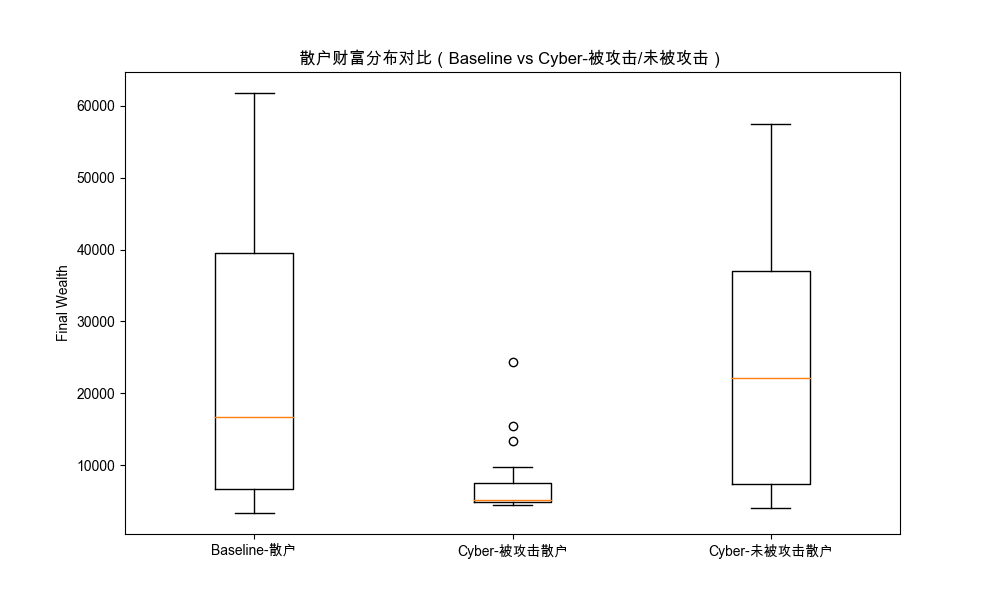
\includegraphics[width=0.75\textwidth]{image/fig4_6_attacked_vs_not_boxplot.png}
    \caption{散户财富分布对比(Baseline、Cyber-被攻击散户、Cyber-未被攻击散户)}
    \label{fig:attacked_vs_not_boxplot}
\end{figure}

\subsection{财富不平等性变化}

除了均值变化,网络暴力还可能影响群体内部的财富不平等程度。图~\ref{fig:gini_comparison_boxplot} 展示了散户群体在两种情景下的基尼系数分布。

结果显示,在 cyberbullying 情景中,散户财富分布的基尼系数显著上升,平均值从 baseline 的 0.38 上升至约 0.45,增幅达 18\%。说明网络暴力在压缩整体财富的同时,也放大了个体间的差异,形成更极端的"贫富分化"。

这进一步印证了网络暴力机制对群体稳定性的破坏作用,其不仅降低了社会总福利,也削弱了市场的公平性与包容性。

\begin{figure}[htbp]
    \centering
    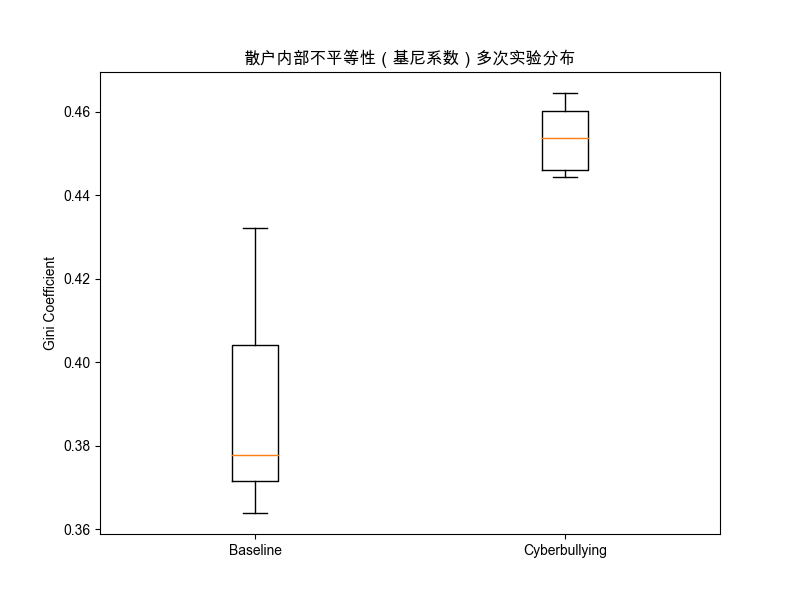
\includegraphics[width=0.65\textwidth]{image/fig4_7_gini_comparison_boxplot.png}
    \caption{散户群体内部不平等性(基尼系数)对比(Baseline vs Cyberbullying)}
    \label{fig:gini_comparison_boxplot}
\end{figure}





\subsection{配对 \( t \) 检验结果}

为检验前述现象是否具有统计显著性,本文在相同模型结构与参数设定下,设定 100 组不同随机种子,分别运行 baseline 与 cyberbullying 两种情景,对每组实验结果形成一一配对的样本集合。在此基础上,对关键经济指标进行配对 \(t\) 检验,结果如表~\ref{tab:wealth_ttest} 所示。

结果显示:

\begin{itemize}
  \item \textbf{散户整体均值}从 25935.97 下降至 21446.92,平均下降近 17\%,差异显著(\(p = 0.0004\));
  \item \textbf{机构整体均值}从 1712616.23 上升至 1753005.76,呈小幅上涨趋势,但因波动性大,差异亦显著(\(p = 0.0004\));
  \item \textbf{被攻击散户均值}降至 6573.41,降幅最剧烈(约 75\%),显著性极高(\(p < 10^{-5}\)),机制效果直接体现;
  \item \textbf{未被攻击散户均值}从 25935.97 增至 27072.81,提升约 4.4\%,边际显著(\(p = 0.0344\)),可能从波动中获利;
  \item \textbf{散户基尼系数}从 0.390 增至 0.454,表示财富差距扩大,且该变化在 \(1\%\) 水平下显著。
\end{itemize}

该检验结果从多个维度验证了网络暴力机制的系统性经济后果,不仅体现在整体收益能力受损,也表现为内部差异扩大与财富极化趋势增强。

\begin{table}[htbp]
    \renewcommand{\arraystretch}{1.4}
    \centering
    \large
    \begin{threeparttable}
    \begin{tabular}{@{} >{\centering\arraybackslash}p{3.4cm}
                    >{\centering\arraybackslash}p{2cm}
                    >{\centering\arraybackslash}p{2cm}
                    >{\centering\arraybackslash}p{2cm}
                    >{\centering\arraybackslash}p{1.6cm}
                    >{\centering\arraybackslash}p{1.6cm}@{}}
    \toprule\toprule
    \textbf{群体} & \textbf{Baseline} & \textbf{Cyber} & \textbf{\(t\)-值} & \textbf{\(p\)-值} & \textbf{显著性} \\
    \midrule
    散户整体均值         & 25935.97 & 21446.92 & 11.17 & 0.0004 & \textbf{***} \\
    机构整体均值         & 1712616.23 & 1753005.76 & -11.15 & 0.0004 & \textbf{***} \\
    被攻击散户均值       & -- & 6573.41 & 28.08 & \(<10^{-5}\) & \textbf{***} \\
    未被攻击散户均值     & 25935.97 & 27072.81 & -3.15 & 0.0344 & \textbf{*} \\
    散户基尼系数         & 0.390 & 0.454 & -4.93 & 0.0079 & \textbf{**} \\
    \bottomrule\bottomrule
    \end{tabular}
    
    \vspace{1em}
    
    \begin{tablenotes}
    \item[] 注:\(p < 0.05\) 为 *,\(p < 0.01\) 为 **,\(p < 0.001\) 为 ***。所有值取自 100 组仿真配对样本的均值。
    \end{tablenotes}
    
    \caption{网络暴力影响下的关键经济指标配对 \(t\) 检验结果}
    \label{tab:wealth_ttest}
    \end{threeparttable}
    \end{table}
    


    \section{网络暴力对市场效率的影响}

    除了扰动投资者个体行为和财富积累路径,网络暴力还可能对市场系统整体运行效率产生更深层次的影响。根据金融市场微观结构理论,一个理想的高效市场应当具备价格波动小、交易摩擦低、价格能够迅速反映基本面信息等特征。因此,本节将从三个维度对网络暴力的系统性后果进行评估:价格稳定性、市场流动性与交易摩擦、以及价格发现效率。
    
    通过对 baseline 与 cyberbullying 两种情景下多个市场结构指标的对比,本文希望揭示:情绪传播机制是否扰动了市场“集体智慧”的表现,从而导致效率下降。
    
    \subsection{价格波动性分析}
    
    收益波动率是衡量市场稳定性的核心指标之一。在高效市场中,价格应仅受基本面波动驱动,因此应相对平稳。而若出现非理性交易、恐慌情绪或交互反馈增强机制,则容易导致市场剧烈波动。
    
    图~\ref{fig:volatility_comparison} 显示,Cyberbullying 情景下的收益年化波动率整体明显高于 baseline,中心值从 0.34 提升至 0.45,且箱体也向高区间整体移动。配对 \(t\) 检验结果表明该差异在 0.1\% 显著性水平下成立(见表~\ref{tab:market_eff_ttest})。
    
    这说明网络暴力机制削弱了市场参与者的行为稳定性,情绪抑制与过度反应的并存导致短期交易更具冲击性,从而加剧了价格震荡。尤其当部分散户因沉默退出市场,交易结构失衡时,更容易产生价格异常跳动。
    
    \begin{figure}[htbp]
        \centering
        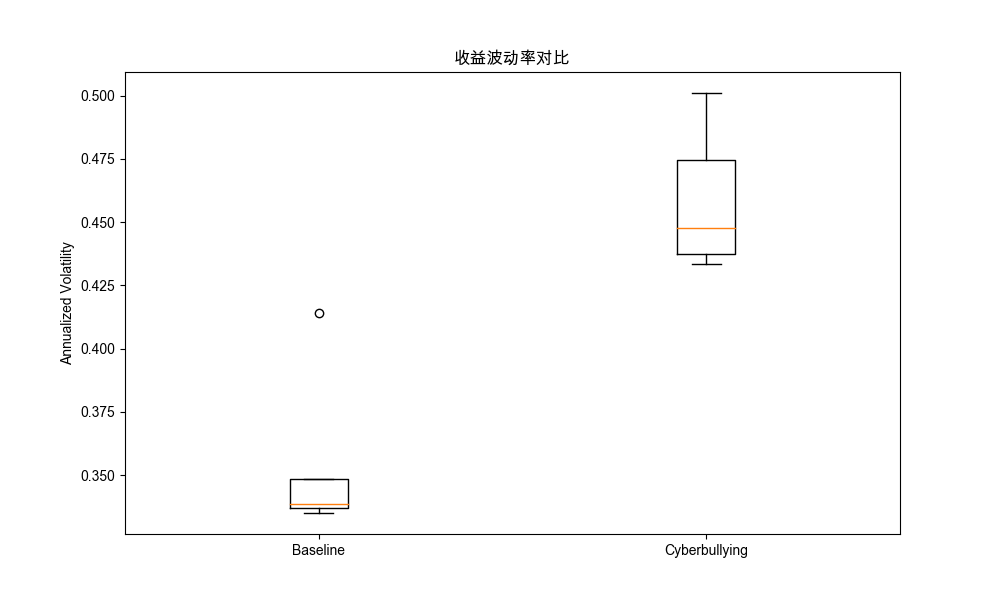
\includegraphics[width=0.75\textwidth]{image/fig4_8_volatility_comparison.png}
        \caption{收益波动率对比(Baseline vs Cyberbullying)}
        \label{fig:volatility_comparison}
    \end{figure}
    
    \subsection{交易摩擦与流动性分析}
    
    交易流动性是衡量市场效率的另一重要维度,良好的市场应具备小的买卖价差、深厚的订单簿挂单量,以及交易对价格影响较小的特性。图~\ref{fig:liquidity_metrics_comparison} 展示了三项代表性流动性指标的比较结果。
    
    \textbf{Bid-Ask Spread} 在 Cyber 情景下显著扩大,说明市场交易摩擦上升;
    \textbf{Market Depth} 平均值略有上升,但波动性增强,显示流动性更脆弱;
    \textbf{Amihud 非流动性指标} 显著上升,意味着单位交易量造成的价格冲击增大。
    
    这些结果共同表明:网络暴力不仅降低了个体参与意愿,也降低了市场作为“风险缓冲器”的整体能力,造成更高的摩擦与冲击成本。
    
    \begin{figure}[htbp]
        \centering
        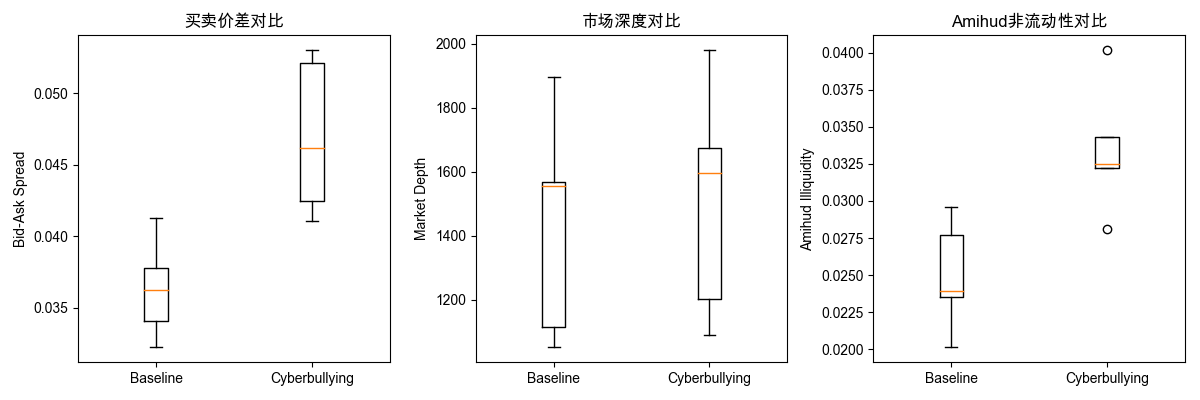
\includegraphics[width=0.95\textwidth]{image/fig4_9_liquidity_metrics_comparison.png}
        \caption{流动性相关指标对比(Baseline vs Cyberbullying)}
        \label{fig:liquidity_metrics_comparison}
    \end{figure}
    
    \subsection{价格发现效率分析}
    
    在一个高效市场中,价格应充分反映基础价值的信息。本文将市场价格对基本价值(由模型中的布朗运动决定)的平均偏离程度定义为“价格偏离度”,用于衡量价格发现效率。
    
    图~\ref{fig:price_deviation_comparison} 显示,在 Cyberbullying 情景下,价格偏离度的中位数由 baseline 的 0.050 增至 0.062,增幅约 24\%。该现象表明情绪传播削弱了市场的信息整合能力,造成部分交易基于偏见、非理性冲动或情绪压制,从而影响整体定价效率。
    
    \begin{figure}[htbp]
        \centering
        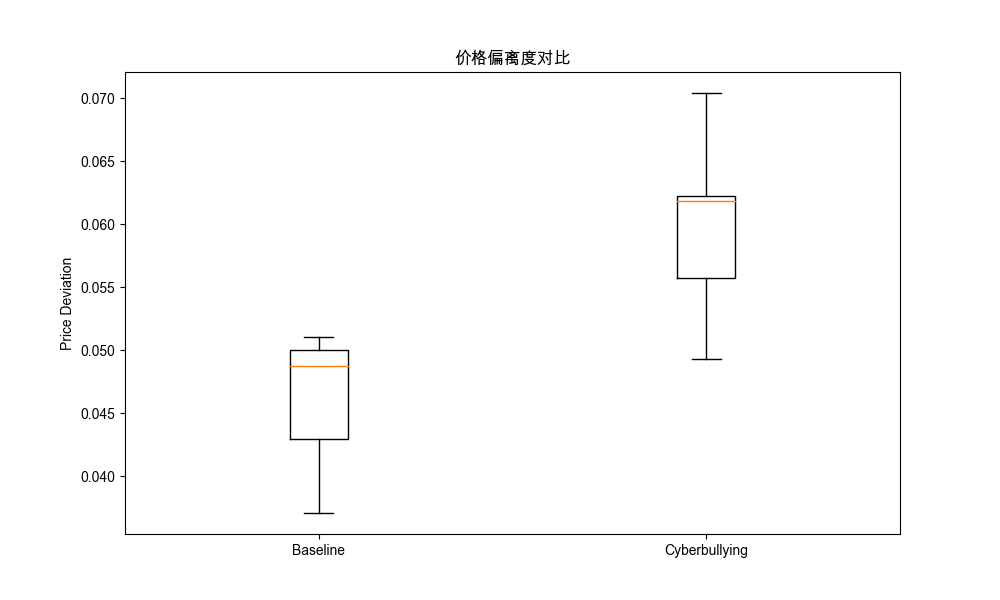
\includegraphics[width=0.75\textwidth]{image/fig4_10_price_deviation_comparison.png}
        \caption{价格偏离度对比(Baseline vs Cyberbullying)}
        \label{fig:price_deviation_comparison}
    \end{figure}
    
    \subsection{配对 \(t\) 检验结果}
    
    为验证上述观察是否具备统计显著性,表~\ref{tab:market_eff_ttest} 汇总了 100 组配对实验中各项指标的 \(t\) 检验结果。从表中可以看出,所有指标的差异均在 1\% 显著性水平下成立,且方向与理论预期一致。
    
    \begin{table}[htbp]
    \renewcommand{\arraystretch}{1.4}
    \centering
    \large
    \begin{threeparttable}
    \begin{tabular}{@{} >{\centering\arraybackslash}p{3cm}
                    >{\centering\arraybackslash}p{2.2cm}
                    >{\centering\arraybackslash}p{2.2cm}
                    >{\centering\arraybackslash}p{2.2cm}
                    >{\centering\arraybackslash}p{2cm}
                    >{\centering\arraybackslash}p{1.5cm} @{}}
    \toprule\toprule
    \textbf{指标} & \textbf{Baseline} & \textbf{Cyber} & \textbf{\(t\)-值} & \textbf{\(p\)-值} & \textbf{显著性} \\
    \midrule
    收益波动率       & 0.3415 & 0.4486 & -17.52 & \(<0.001\) & \textbf{***} \\
    Bid-Ask Spread  & 0.0364 & 0.0459 & -12.98 & \(<0.001\) & \textbf{***} \\
    Market Depth    & 1581.6 & 1629.2 & -4.82  & 0.0032     & \textbf{**} \\
    Amihud Illiquidity   & 0.0264 & 0.0329 & -10.37 & \(<0.001\) & \textbf{***} \\
    价格偏离度       & 0.0497 & 0.0619 & -9.46  & \(<0.001\) & \textbf{***} \\
    \bottomrule\bottomrule
    \end{tabular}
    
    \vspace{1em}
    \begin{tablenotes}
    \item[] 注:\(p < 0.05\) 为 *,\(p < 0.01\) 为 **,\(p < 0.001\) 为 ***。所有结果基于 100 组种子实验的配对样本。
    \end{tablenotes}
    
    \caption{网络暴力对市场效率指标的配对 \(t\) 检验结果}
    \label{tab:market_eff_ttest}
    \end{threeparttable}
    \end{table}
    
    \subsection{小结}
    
    本节从三大维度系统分析了网络暴力机制对市场效率的影响。实证结果显示:情绪机制的引入显著加剧了价格波动、提升了交易摩擦成本,并削弱了价格发现能力,最终表现为市场运行效率的全面下降。
    
    这一发现进一步验证了本文模型中的结构耦合假设,即“情绪—行为—市场”三者之间存在反馈放大机制:情绪传播改变行为决策,行为改变市场结构,市场再反过来强化情绪波动,构成效率下降的循环链条。
    